\documentclass[a4paper,12pt]{ltjsarticle}

% ===== Fonts & Language =====
\usepackage[haranoaji,nfssonly]{luatexja-preset}

% ===== Layout (margins tightened for 12pt) =====
\usepackage[top=15mm,bottom=15mm,left=18mm,right=18mm]{geometry}
\usepackage{fancyhdr}
\usepackage{titlesec}
\usepackage{multicol}
\usepackage{enumitem}
\usepackage{float}

% ===== Graphics & Color =====
\usepackage{graphicx}
\usepackage{xcolor}
\usepackage{tikz}
\usetikzlibrary{calc,positioning,arrows.meta,shapes.geometric,decorations.pathreplacing}
\usepackage[most]{tcolorbox}
\usepackage{wrapfig}

% ===== Tables =====
\usepackage{booktabs}
\usepackage{tabularx}
\usepackage{array}

% ===== Hyperlinks =====
\usepackage{hyperref}
\hypersetup{colorlinks=true,linkcolor=blue!60!black,urlcolor=blue!60!black,citecolor=blue!60!black}

% ===== Color definitions =====
\definecolor{mainblue}{HTML}{1A5276}
\definecolor{accentorange}{HTML}{E67E22}
\definecolor{lightbg}{HTML}{F4F6F7}
\definecolor{successgreen}{HTML}{27AE60}
\definecolor{dangerred}{HTML}{E74C3C}
\definecolor{sectionblue}{HTML}{2C3E50}

% ===== Section formatting =====
\titleformat{\section}
  {\large\bfseries\sffamily\color{mainblue}}
  {\thesection}{0.6em}{}
  [\vspace{-0.5em}\textcolor{mainblue}{\rule{\textwidth}{1pt}}]

\titleformat{\subsection}
  {\large\bfseries\sffamily\color{sectionblue}}
  {\thesubsection}{0.6em}{}

\titleformat{\subsubsection}
  {\normalsize\bfseries\sffamily\color{sectionblue}}
  {\thesubsubsection}{0.5em}{}

\titlespacing*{\section}{0pt}{0.6em}{0.3em}
\titlespacing*{\subsection}{0pt}{0.4em}{0.15em}
\titlespacing*{\subsubsection}{0pt}{0.2em}{0.08em}

% ===== Custom boxes =====
\newtcolorbox{keybox}[1][]{
  colback=mainblue!5,colframe=mainblue,
  fonttitle=\bfseries\sffamily,
  title=#1,boxrule=0.8pt,arc=2pt,
  left=3pt,right=3pt,top=2pt,bottom=2pt
}

\newtcolorbox{highlightbox}{
  colback=accentorange!8,colframe=accentorange,
  boxrule=0.8pt,arc=2pt,
  left=3pt,right=3pt,top=2pt,bottom=2pt
}

\newtcolorbox{graybox}{
  colback=lightbg,colframe=lightbg!60!gray,
  boxrule=0.4pt,arc=2pt,
  left=3pt,right=3pt,top=2pt,bottom=2pt
}

% ===== Header / Footer =====
\pagestyle{fancy}
\fancyhf{}
\renewcommand{\headrulewidth}{0.4pt}
\fancyhead[L]{\small\sffamily\color{gray}未踏IT人材発掘・育成事業 提案書}
\fancyhead[R]{\small\sffamily\color{gray}無限問題作成AI「モンジェネ」}
\fancyfoot[C]{\small\sffamily\color{gray}\thepage\,/\,10}

% ===== List spacing =====
\setlist{nosep,leftmargin=1.2em,topsep=0pt,partopsep=0pt}
\setlist[itemize]{label={\color{mainblue}\textbullet}}

% ===== Paragraph =====
\setlength{\parindent}{1em}
\setlength{\parskip}{0pt}

% ============================================================
\begin{document}

% ===== COMPACT HEADER (no separate title page) =====
\noindent
\begin{minipage}[t]{0.62\textwidth}
\vspace{0pt}
{\large\sffamily\bfseries\color{mainblue} 生徒ごとに個別最適化された問題生成システムの開発}\\[2pt]
{\normalsize\sffamily\color{accentorange} 無限問題作成AI「モンジェネ」}\\[4pt]
{\small\sffamily
\textbf{申請者:} 高橋創真（長岡技術科学大学大学院 修士1年）\\
\textbf{共同開発者:} 若月耕紀（長岡技科大 院M1）、小武壮太（長岡技科大 院M1）、舛田岳（新潟大 院M1）
}
\end{minipage}
\hfill
\begin{minipage}[t]{0.35\textwidth}
\vspace{0pt}
\begin{tcolorbox}[colback=lightbg,colframe=mainblue,arc=2pt,boxrule=0.6pt,
  left=3pt,right=3pt,top=2pt,bottom=2pt]
\small\sffamily
生徒の手書き答案をAIで解析し、間違え方や苦手を抽出し、それらを克服できる問題を\textbf{無限に}生成する。「問題生成」と「採点」のサイクルにより、これまでにない学習効果を実現する。
\end{tcolorbox}
\end{minipage}


{\color{mainblue}\rule{\textwidth}{1.2pt}}
\vspace{0.5em}

% ============================================================
% ① なにをつくるか
% ============================================================
\section{なにをつくるか}

\subsection{背景}

「問題を探している時間で、もっと生徒に教えたいな……」---私の5年間の塾講師経験で、何度もそう感じてきた。

私が勤める個別指導塾では、先生1人に生徒2人、1コマ80分で指導する。1人の生徒に割ける時間は実質\textbf{40分}。この40分のうち、問題集から適切な問題を探す作業に\textbf{約10分}---指導時間の25\%が「紙をめくる時間」に消えてしまう。しかも、やっと見つけた問題が生徒の苦手にマッチしているかはわからない。私は約30人の生徒を受け持ち、月ごとに統一模試の結果を見ながら個別に対応するが、30人全員の苦手を正確に把握し続けることは人間の記憶力では限界がある。しかも\textbf{単元が変わるたびに苦手な生徒が入れ替わる}。先月「方程式」で苦戦した生徒が今月は問題なく、代わりに別の生徒が「図形」で躓く---この動的なバラつきへの対応は5年の経験でも容易ではない。

私は塾講師80名を束ねるリーダーとして同僚を指導するなかで、同じ悩みを持つ講師が多いことを実感している。そこで私たちは、問題を探すのではなく「作ってしまえばいい」と考え、経産省AKATSUKI事業 ETSUZAN（新潟県版未踏的人材育成事業）にて、無限問題生成AI「モンジェネ」を開発した。

\begin{figure}[H]
  \centering
  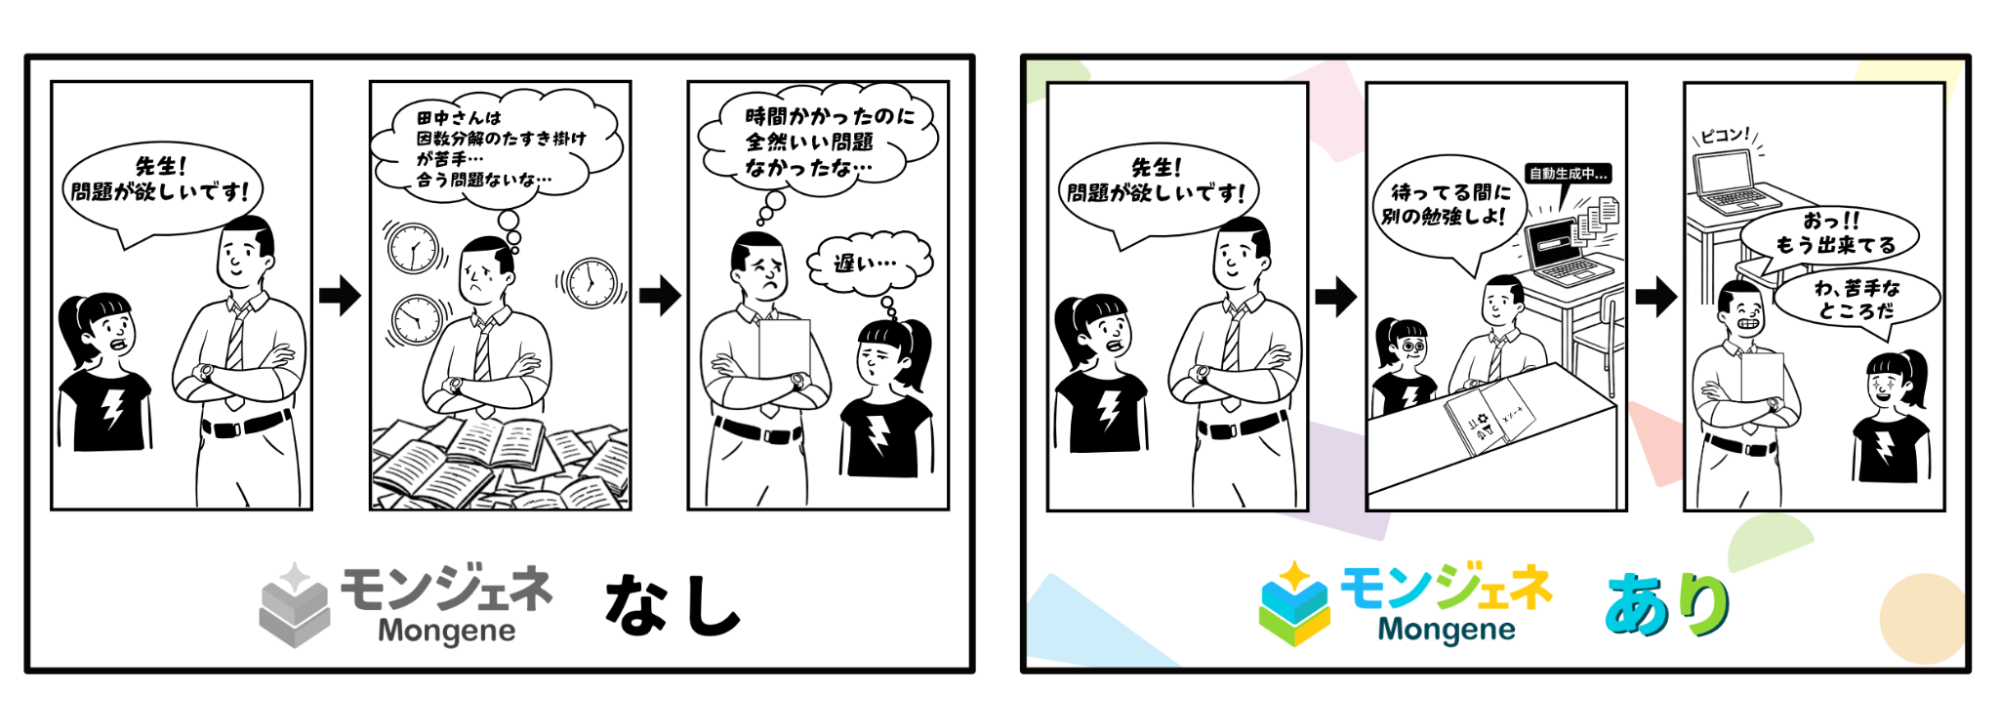
\includegraphics[width=0.75\textwidth]{mongene-compare.png}
  \caption{モンジェネの提供価値：問題探しの時間を問題生成に置き換え、講師が生徒と向き合う時間を最大化する}
  \label{fig:manga}
\end{figure}

\subsubsection{ETSUZANでの成果と課題}

モンジェネは、解き直したい問題を入力すると3パターンの類似問題を出力するWebアプリである。

\begin{itemize}
  \item \textbf{パターンA：}数値のみ変更（ケアレスミス克服用）
  \item \textbf{パターンB：}文脈を変更（公式・定理の定着確認用）
  \item \textbf{パターンC：}問われる内容が異なる（解法戦略の強化用）
\end{itemize}

数値計算精度や図形描画精度の課題に対しては、LLMで直接生成するのではなくPythonコードを生成・外部実行する方式を採用し、「会話なしに一気に問題を作成できる」仕組みを実現した。

しかし、2026年1月〜3月の受験期に毎日モンジェネを使い込んだところ、\textbf{まだまだ足りない}と痛感した。難易度の調整ができない、出力は固定の3パターンのみ、そして何より---生徒一人ひとりの苦手が反映されていない。塾講師から\textbf{「生徒ごとの苦手が反映された問題があれば」}という声が挙がり、これが本提案の出発点となった。

近年、LLMを活用した教育システムの研究が急速に進展しており\,[6]、AI駆動型ITSはK-12教育で一貫してポジティブな学習効果が確認されている\,[7]。LLMを用いた数学的エラーの自動分類も、専門家一致度F1スコア85\%超を達成した\,[8]。

\subsection{提案システム}

本システムは、\textbf{「採点・苦手分析」→「教師へのフィードバック＋対策問題生成」→「生徒が解く」}のサイクルを繰り返すことで、生徒の学力を着実に向上させる。


\begin{keybox}[学術的根拠：Bloomの完全習得学習]
教育心理学者 B.\,Bloom\,(1984) は、完全習得学習と1対1個別指導を組み合わせると、平均的な生徒が\textbf{上位2\%}の成績に到達する（2$\sigma$効果）と報告した\,[1]。近年、生成AIがこの2シグマ問題に対するスケーラブルな解決策となり得ることが実証されている\,[2]。本システムは、このサイクルをAIで自動化し、\textbf{1対1個別指導の効果を1対多の塾環境で再現する}ことを目指す。
\end{keybox}


本提案は\textbf{2つの柱}を掲げる。

\begin{highlightbox}
\begin{enumerate}[leftmargin=2em]
  \item \textbf{個別最適化（パーソナライズ）}：生徒一人ひとりの苦手を高解像度で分析し、その苦手にピンポイントの問題を無限に生成する。
  \item \textbf{完全習得学習（マスタリーラーニング）}：できるようになるまで問題が出てくる。知識グラフで前提概念を管理し、根本原因から段階的に積み上げる。
\end{enumerate}
\end{highlightbox}

\begin{figure}[H]
  \centering
  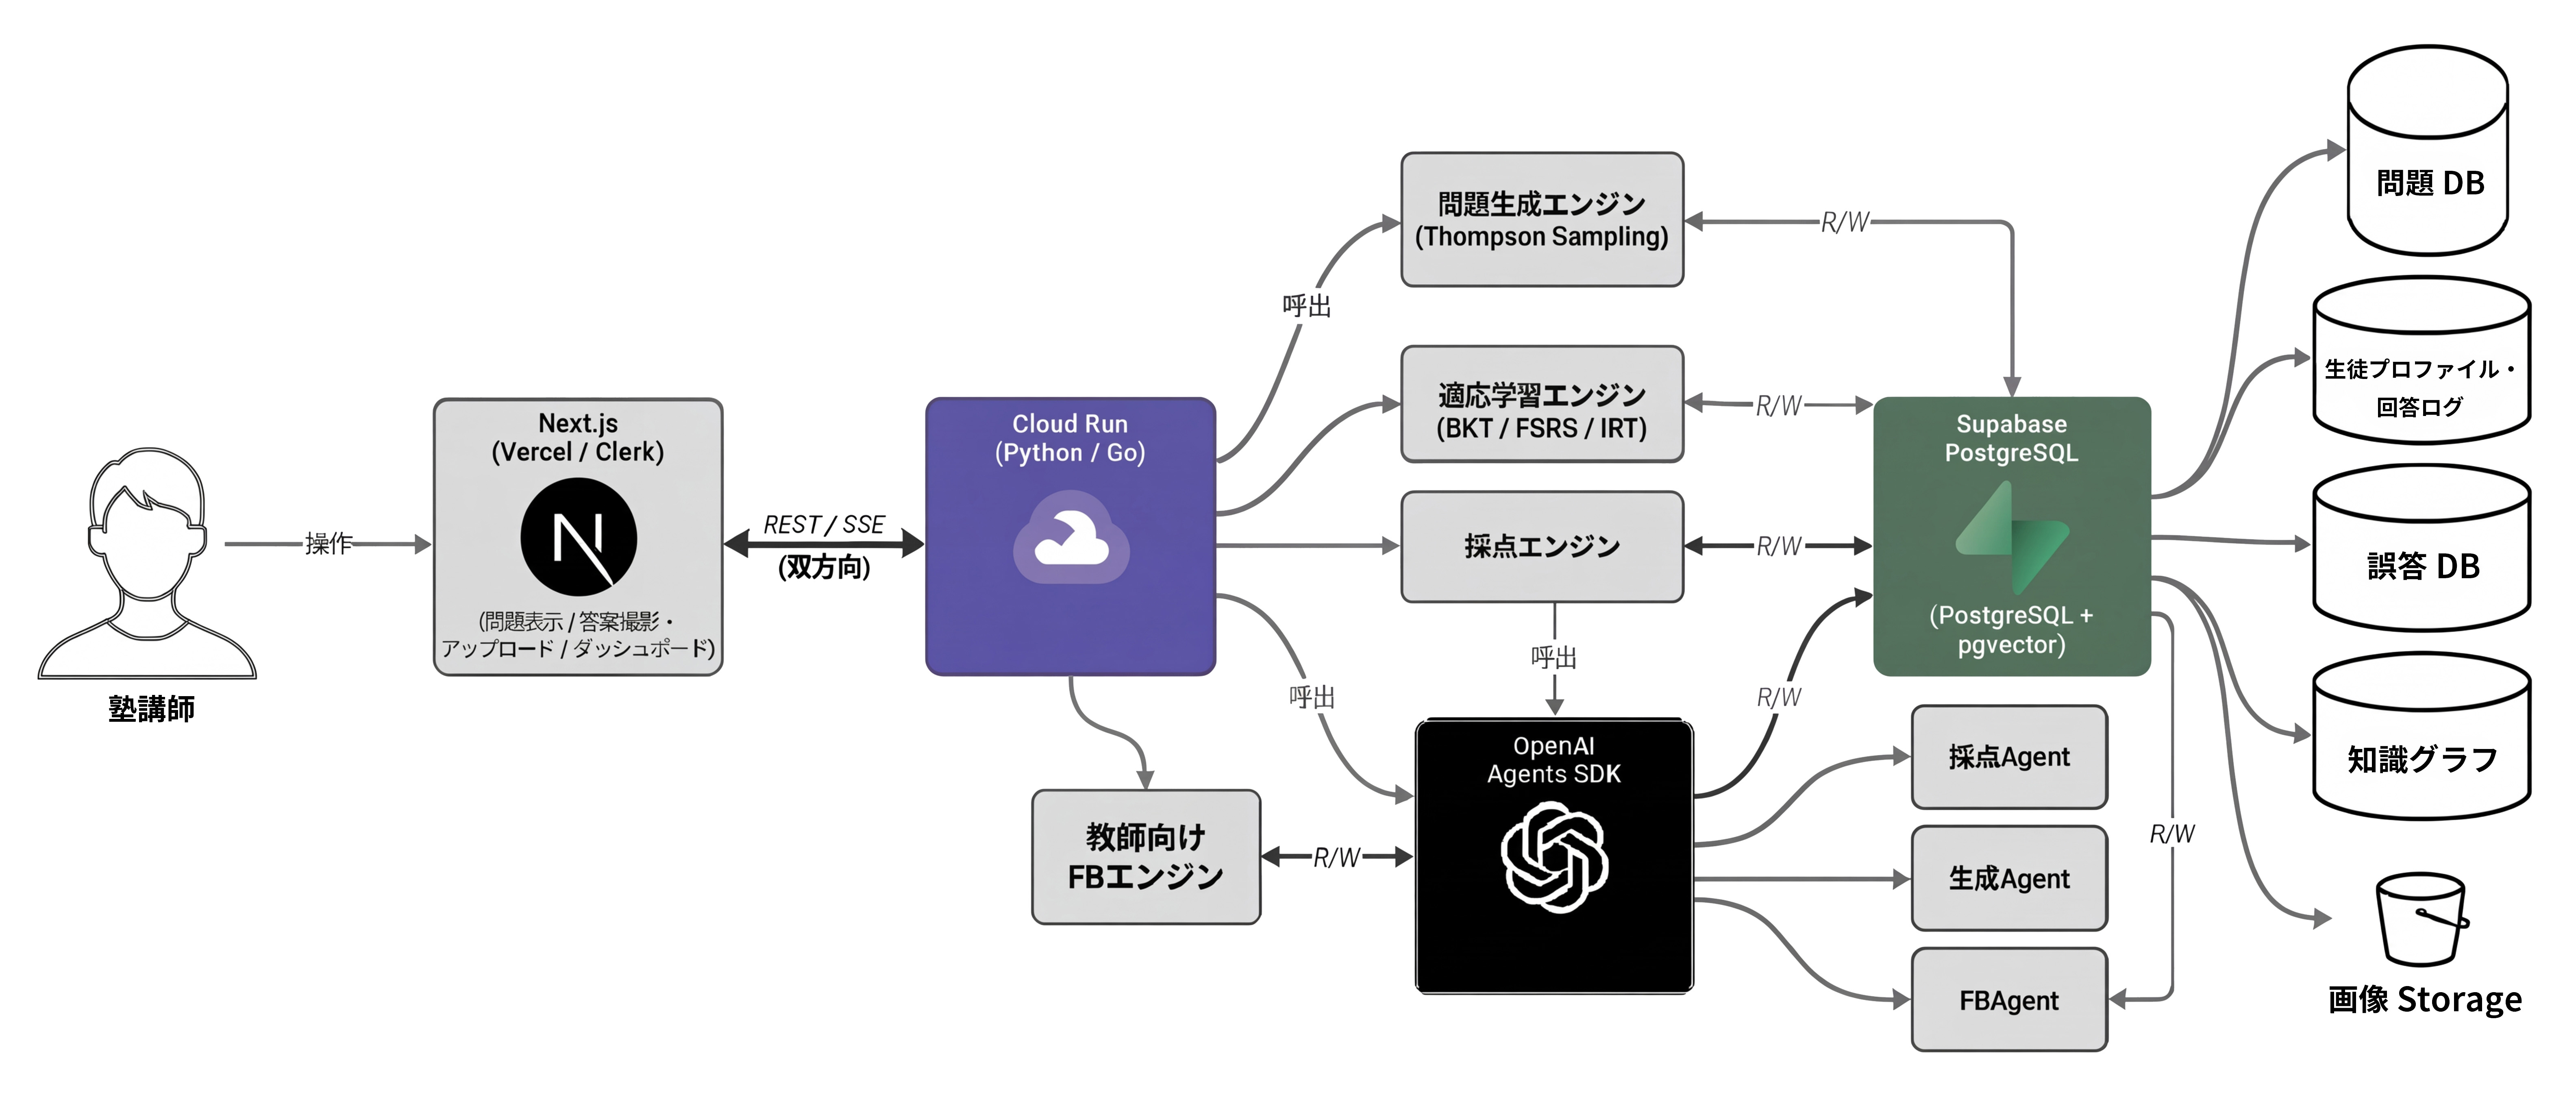
\includegraphics[width=0.9\textwidth]{system-arch-new.jpg}
  \caption{システム構成図：フロントエンド・バックエンド・AI Agent・データベースの全体構成}
  \label{fig:system_overview}
\end{figure}

以下に、図\ref{fig:system_overview}に示した各コンポーネントの概要を述べる。

\begin{itemize}
  \item \textbf{採点Agent}：GPT-5.4 Vision＋OpenAI Agents SDKで手書き答案を読み取り、途中式レベルの自動採点を行う。最大1,024万画素の高解像度入力に対応。Code Interpreterで答案に直接赤ペン添削を書き込み、間違いを4種類に自動分類する。
  \item \textbf{問題生成Agent}：LLM（GPT-5.4 / Claude）＋Code Interpreterで数学的に正確な問題を生成。SymPyで計算検証、Matplotlibで図形描画。苦手プロファイルに基づく個別最適化問題を生成する。
  \item \textbf{知識グラフ}：数学の概念間の前提関係をDAGとして定義。つまずいた際にグラフを遡り根本原因を特定、段階的な学習パスを自動決定する。
  \item \textbf{適応学習エンジン}：BKTで概念ごとの習得確率を推定し、習得度85\%を基準に移行判定。FSRS v6で最適な復習タイミングを決定。
  \item \textbf{問題DB}：統一模試データからIRTで難易度を較正。LightGBMによる難易度推定と埋め込みベクトル（768次元）のセマンティック検索を統合。Supabase（PostgreSQL + pgvector）上に構築。
  \item \textbf{苦手プロファイル}：採点結果・エラー分類・習得確率を生徒ごとに蓄積。時系列のエラー推移を追跡し、問題生成とFBの両方に活用。
  \item \textbf{教師向けFBダッシュボード}：苦手ランキング・エラー推移・指導アクションを自動生成。講師が修正を返す双方向ループでシステム精度を継続改善。
\end{itemize}

以下、各機能の詳細を述べる。

\subsubsection{【採点・苦手分析エンジン】}

\noindent\textbf{入力：}問題文＋正答、生徒の手書き答案\quad\textbf{出力：}正誤判定、途中式フィードバック、エラー分類

生徒の手書き答案をLLMで採点し、「どのステップで間違えたか」を特定する。間違いのタイプを以下の4種類に自動分類する。


\begin{footnotesize}\noindent
\begin{tabularx}{\linewidth}{>{\bfseries}l X X}
\toprule
エラー分類 & 内容 & 具体例 \\
\midrule
読解・理解エラー & 問題文の読み間違い、求めるものの取り違え & 面積と体積を取り違え \\
変換エラー & 問題を数式に変換する段階でのミス & 「3倍より2大きい」を$3x-2$とする \\
処理エラー & 正しい方針だが計算過程でミス & 移項時の符号ミス、公式の記憶違い \\
書き写しエラー & 途中は正しいが最終解答の転記ミス & 正しい値を途中で出しているのに誤記 \\
\bottomrule
\end{tabularx}
\end{footnotesize}


このエラー分類により、間違いの本質が「公式を\textbf{知らない}」のか「\textbf{忘れている}」のか「\textbf{使い方がわからない}」のかを区別する。この区別が、次の問題生成の精度を決定づける。

採点結果は蓄積型の\textbf{苦手プロファイル}として記録する。概念ごとの習得確率をBayesian Knowledge Tracing\,[3]で追跡し、LLMとの統合によりコールドスタート問題を解決する\,[4]。習得確率が85\%を超えた概念を「習得済み」と判定する。

\subsubsection{【教師向けフィードバック】}

塾講師にとって必要なのは「次の授業で何を教えるべきか」の判断材料である。本システムは以下を自動生成する。

\begin{itemize}
  \item \textbf{苦手ランキング（優先順位付き）}---志望校の出題傾向を加味して克服すべき苦手を優先順位付け
  \item \textbf{エラーパターンの推移}---直近数週間で「計算ミスは減少」「概念誤解が増加」等のトレンド分析
  \item \textbf{具体的な指導アクション}---「空間図形は展開図から復習が必要」等の具体的提案
\end{itemize}

さらに、塾講師はフィードバックに対して\textbf{修正・補足を返す}ことができる。この「FBに対するFB」がデータベースに蓄積され、システムの分析精度を継続的に改善する。塾講師の経験知をシステムに還元する双方向ループである。

\subsubsection{【個別最適化問題生成エンジン】}

ETSUZANの3パターン生成を基盤とし、苦手プロファイルに基づく3つのモードに拡張する。


\begin{footnotesize}\noindent
\begin{tabularx}{\linewidth}{>{\bfseries}l X}
\toprule
モード & 内容 \\
\midrule
苦手克服 & 採点で特定された苦手にピンポイントの問題を生成。知識グラフを遡り根本原因から対処 \\
段階的ステップアップ & 概念ごとに習得度85\%達成まで出題を継続。完全習得学習のAI実装 \\
模試対策 & 志望校の出題傾向・難易度構成を解析し、\textbf{本番と同一構成の模擬テスト一式}を自動生成 \\
\bottomrule
\end{tabularx}
\end{footnotesize}


個別最適化問題の生成では、「元の問題文」「模範解答」「生徒の手書き答案」「採点フィードバック」の\textbf{4点をLLMに入力}し、エラー分類に応じた矯正問題を生成する。問題の提供は\textbf{DB検索とLLM新規生成のハイブリッド}で行い、Thompson Samplingにより探索と活用のバランスを最適化する。生成問題はPythonコード実行による数学的検証を経てから出題する。

\subsubsection{【完全習得学習の仕組み】}

生徒が確実にできるようになるまで、以下の判定基準でサイクルを繰り返す。

\begin{graybox}
\textbf{習得判定の3条件:}
\begin{enumerate}[leftmargin=2em]
  \item 概念ごとの習得確率（Bayesian Knowledge Tracing）が\textbf{85\%以上}
  \item 直近5問の正答率が\textbf{80\%以上}
  \item \textbf{3問以上}の連続正答
\end{enumerate}
3条件を満たした概念は「習得済み」→次の概念へ。満たさない場合は矯正問題を自動提供。
\end{graybox}

数学の概念には前提関係がある。この前提関係を\textbf{知識グラフ}（有向非巡回グラフ）として管理する。


\begin{figure}[H]
\centering
\begin{tikzpicture}[
  node distance=0.5cm and 1.5cm,
  mastered/.style={rectangle, rounded corners=3pt, draw=successgreen, fill=successgreen!10,
    font=\footnotesize\sffamily, minimum height=0.8cm, minimum width=2.2cm, align=center, line width=0.8pt},
  weak/.style={rectangle, rounded corners=3pt, draw=dangerred, fill=dangerred!10,
    font=\footnotesize\sffamily, minimum height=0.8cm, minimum width=2.2cm, align=center, line width=0.8pt},
  progress/.style={rectangle, rounded corners=3pt, draw=accentorange, fill=accentorange!10,
    font=\footnotesize\sffamily, minimum height=0.8cm, minimum width=2.2cm, align=center, line width=0.8pt},
  arr/.style={-{Stealth[length=5pt,width=4pt]}, thick, color=gray!60},
  every node/.append style={inner sep=4pt}
]
  % 横一列に並べる
  \node[mastered] (sqrt) {平方根\\[-1pt]{\scriptsize\bfseries\color{successgreen}習得 92\%}};
  \node[weak, right=of sqrt] (factor) {因数分解\\[-1pt]{\scriptsize\bfseries\color{dangerred}習得 38\%}};
  \node[weak, right=of factor] (quad) {二次方程式\\[-1pt]{\scriptsize\bfseries\color{dangerred}習得 25\%}};
  \node[weak, right=of quad] (space) {空間図形\\[-1pt]{\scriptsize\bfseries\color{dangerred}習得 12\%}};

  % 下段：三平方の定理
  \node[progress, below=0.8cm of $(factor)!0.5!(quad)$] (pyth) {三平方の定理\\[-1pt]{\scriptsize\bfseries\color{accentorange}習得 65\%}};

  % 矢印
  \draw[arr] (sqrt) -- (factor);
  \draw[arr] (sqrt) -- (pyth);
  \draw[arr] (factor) -- (quad);
  \draw[arr] (pyth) -- (space);
  \draw[arr] (quad) -- (space);

  % 凡例（グラフ下部中央に配置）
  \node[font=\scriptsize\sffamily, anchor=north] at ($(factor.south)+(0,-1.6)$) {%
    \textcolor{successgreen}{\rule{6pt}{6pt}}\,習得済\quad
    \textcolor{accentorange}{\rule{6pt}{6pt}}\,学習中\quad
    \textcolor{dangerred}{\rule{6pt}{6pt}}\,苦手};
\end{tikzpicture}
\caption{知識グラフの例：空間図形（習得12\%）でつまずいた生徒の根本原因を因数分解（38\%）まで遡り、そこから段階的に習得させる。}
\label{fig:knowledge_graph}
\end{figure}
\vspace{-0.5em}

生徒がつまずいた場合、知識グラフを遡って根本原因を特定する。空間図形でつまずいている生徒の真の原因が三平方の定理や因数分解の理解不足であれば、まずそこに戻って習得させてから進む。国内3,200以上の塾で導入されているatama+の「根本原因分析」と同様のアプローチだが、モンジェネはAIによる\textbf{無限の問題生成}と\textbf{紙の手書き答案への対応}という独自の強みを持つ。

\subsubsection{【データベース---競争優位の源泉】}

本システムの長期的な競争優位は、蓄積される独自データベースにある。


\begin{footnotesize}\noindent
\begin{tabularx}{\linewidth}{>{\bfseries}l X}
\toprule
データ層 & 内容と意義 \\
\midrule
第1層：原データ & 統一模試協会の大規模問題データ（正答率付き）、各県入試問題。提携なしには入手不可能 \\
第2層：アノテーション & 塾講師が検証した難易度ラベル（正答率5\%刻み21段階）、公式タグ、誤答パターン。LLM構造化出力＋人間検証で構築 \\
第3層：学習効果 & どの問題がどの苦手パターンの生徒に効果があったか。使うほど精度が上がるフライホイール効果 \\
\bottomrule
\end{tabularx}
\end{footnotesize}


DBに蓄積された問題は埋め込みベクトルによるセマンティック検索に対応し、「この生徒の苦手に最も適した問題」を高速に発見する。統一模試データからIRT（項目反応理論）パラメータを較正し、難易度の客観的評価を実現する。後発の競合がシステムを模倣しても、このデータ蓄積は即座に再現できない。


\noindent\textbf{データの好循環（フライホイール効果）：}生徒が問題を解く→回答データ蓄積→IRT較正精度向上→問題推薦精度向上→学習効果向上→ユーザー増加→さらにデータ蓄積。時間が経つほど価値が加速度的に高まる。

\subsection{未踏期間中の目標}

\begin{enumerate}[leftmargin=2em]
  \item 生徒の手書き答案を採点し、間違えたステップとエラータイプを自動抽出する
  \item 苦手プロファイルに基づく個別最適化問題を生成する
  \item 採点→問題生成のサイクルを塾の現場で実証実験し、学習効果を検証する
\end{enumerate}

% ============================================================
\section{どんな出し方を考えているか}

\subsection{公開方法}

Webアプリケーション「モンジェネ」として公開する。塾で用いるタブレット端末やPCでの使用を想定しており、幅広いハードウェアに対応可能なWebアプリが最適である。生徒の手書き答案はスマートフォンやタブレットのカメラで撮影し、アップロードする。紙のワークフローを完全に維持したまま、AIの恩恵を受けられる設計である。

\subsection{ターゲットと展開戦略}

\textbf{未踏期間中}は、提案者代表の高橋が所属する個別指導塾（講師80名・生徒約500名）に限定して検証する。ETSUZAN期間で実証実験を行っており、校長の承認も得ている。ユーザーの声を聞きながらUI/UXを磨き込み、その後の展開に備える。

\textbf{未踏期間後}は、2つのフェーズで展開する。

\begin{enumerate}[leftmargin=2em]
  \item \textbf{Phase 1（地域展開）}：同地域の塾への横展開。新潟県公立高校入試に特化した問題データベースと志望校別の出題傾向分析が差別化要素となる。
  \item \textbf{Phase 2（全国展開）}：各都道府県の入試問題・統一模試データをDBに取り込み、地域ごとの特徴を反映させた全国対応版を提供する。
\end{enumerate}

\subsection{学術的な発表・未踏後のアクション}

ユーザーの負担軽減が主目的だが、実証実験で得られる学習効果の定量データに学術的価値を見出した際は、教育工学系の学会（日本教育工学会、AIED等）への投稿を積極的に行う。

未踏に応募する理由は、\textbf{PMの指導のもとで技術を磨き、未踏コミュニティの力を借りて展開を加速したい}からである。自分の塾だけなら未踏なしでも開発を続けられるが、全国の塾に展開するためには、PM・先輩クリエータからのフィードバックと、未踏ブランドによる信頼獲得が不可欠だと考えている。未踏期間後は未踏アドバンストへの進出も視野に入れる。

% ============================================================
\section{斬新さの主張、期待される効果}

\subsection{斬新さ---既存サービスとの本質的な違い}

国内EdTech市場にはatama+（4,500教室導入）やQubena（100万人以上）といった先行サービスが存在する。しかし、これらは\textbf{タブレット完結型}であり、問題供給はDB内の既存問題の\textbf{検索・提供}にとどまる。モンジェネは知識グラフを用いて生徒の根本原因を特定した上で、その苦手に特化した問題をLLMで\textbf{動的に生成}するという本質的な違いがある。


\begin{footnotesize}\noindent
\begin{tabularx}{\linewidth}{>{\bfseries}l X X}
\toprule
比較軸 & atama+\,/\,Qubena & モンジェネ（本提案） \\
\midrule
入力方式 & タブレット操作のみ & \textbf{紙の手書き答案OK} \\
問題供給 & 自社DB内の既存問題を選択 & \textbf{AIが無限に新規生成} \\
エラー分析 & 正誤＋解答時間＋迷い挙動 & \textbf{途中式レベルの4種類分類} \\
講師の役割 & 見守り（コーチ） & \textbf{主役（AIのFBを元に解説）} \\
講師の知見還元 & なし（一方通行） & \textbf{FBへのFBでDB改善} \\
導入コスト & 高い（タブレット＋月額） & \textbf{低い（紙＋撮影＋従量課金）} \\
\bottomrule
\end{tabularx}
\end{footnotesize}


\begin{highlightbox}
\textbf{一言で表すなら}：atama+は「タブレットの中の完璧な先生」、モンジェネは「紙の現場に溶け込むAIアシスタント」。既存の紙ベースの指導を活かしたまま、採点と問題生成という最も時間のかかる作業をAIが肩代わりする。塾の指導モデルを置き換えるのではなく、\textbf{講師が生徒と向き合う時間を最大化する}。
\end{highlightbox}

\noindent
加えて、\textbf{開発者自身が5年間の塾講師}であり、「生徒がどこでつまずくか」という肌感覚がシステム設計に直接反映されている点が、技術だけでは到達できない本提案の強みである。

\subsection{期待される効果}

\begin{itemize}
  \item \textbf{生徒の学力向上}：AI駆動型ITSのシステマティックレビュー\,[7]では、従来の教師主導指導に対し中〜大の効果量で優位性が確認されている。生成AIチューターは対面指導の2倍の学習効率を数百分の一のコストで達成した事例もある\,[2]。本システムの学習効果を実証実験で検証する。
  \item \textbf{講師の負担軽減}：1コマ40分のうち問題探しに費やす約10分を1分以下に短縮し、\textbf{指導時間を25\%増加}させる。講師80名に展開すれば、塾全体で月間数百時間の指導時間が生まれる計算となる。
  \item \textbf{教育格差の縮小}：1対1の個別指導は高コストだが、AIがその品質を1対多で再現することで、経済的理由で質の高い指導を受けられなかった生徒にも届けられる。
\end{itemize}

\subsection{先行事例との効果の比較}

類似のAI教育システムの実績として、以下が報告されている。
\begin{itemize}
  \item \textbf{Qubena}（COMPASS社）：経済産業省の実証事業において、中学校数学の標準授業時間62時間分を\textbf{34時間で完了}し、かつ理解度・テスト得点は向上した。
  \item \textbf{atama+}：長野県のある塾で、国公立大学合格者が2020年度の6名から2024年度の\textbf{42名へ約7倍}に増加した事例が報告されている。
\end{itemize}

これらはタブレット完結型のシステムであるが、モンジェネは紙ベースの現場に適用可能な点で\textbf{より広い対象に展開できるポテンシャル}を持つ。

なお、LLMを用いた教育システムに関する最新のサーベイ\,[6]を精査した上で、「知識グラフによる根本原因分析」と「LLMによる問題の動的生成」を\textbf{紙の手書き答案}に対して統合的に適用するシステムは、国内外の学術研究・商用サービスを含めて確認されていない。

% ============================================================
\section{具体的な進め方と予算}

\subsection{技術スタックと開発体制}


\begin{footnotesize}\noindent
\begin{tabularx}{\linewidth}{>{\bfseries}l X}
\toprule
領域 & 技術 \\
\midrule
バックエンド & Go (Golang), Python, FastAPI \\
フロントエンド & TypeScript, Next.js \\
AI/ML & OpenAI API (GPT-5.4), Gemini API, Bayesian Knowledge Tracing, FSRS v6 \\
インフラ/DB & AWS or GCP, Supabase (PostgreSQL + pgvector), Vercel \\
認証/決済 & Clerk, Stripe \\
デザイン & Figma \\
\bottomrule
\end{tabularx}
\end{footnotesize}

\subsection{開発チームと役割分担}


\begin{footnotesize}\noindent
\begin{tabularx}{\linewidth}{>{\bfseries}l l X}
\toprule
氏名 & 所属 & 担当 \\
\midrule
高橋創真 & 長岡技科大 院M1 & チームマネジメント、ユーザヒアリング、要件定義 \\
若月耕紀 & 長岡技科大 院M1 & フロントエンド・バックエンド実装全般 \\
小武壮太 & 長岡技科大 院M1 & UI/UXデザイン、システムデザイン \\
舛田　岳 & 新潟大 院M1 & LLM・ML・インフラ/システム開発全般 \\
\bottomrule
\end{tabularx}
\end{footnotesize}

\subsection{開発スケジュール}

\begin{footnotesize}\noindent
\begin{tabularx}{\linewidth}{>{\bfseries}l X}
\toprule
期間 & マイルストーン \\
\midrule
M1--M2 & 採点エンジンの精度向上。手書き答案のエラー分類精度を検証。統一模試データの取り込みとDB基盤構築 \\
M3--M4 & 苦手プロファイル蓄積機能の実装。知識グラフ（数学の前提概念DAG）構築。塾講師によるアノテーション開始 \\
M5--M6 & 個別最適化問題生成エンジン実装。BKT・FSRSによる適応的出題。LLM生成問題の数学的検証パイプライン構築 \\
M7--M8 & 教師向けFBダッシュボード実装。完全習得学習フロー（マスタリー判定・矯正問題自動生成）の統合 \\
M8--M9 & 塾での実証実験（講師80名・生徒500名規模）。A/Bテストによる学習効果の定量評価と改善サイクル \\
\bottomrule
\end{tabularx}
\end{footnotesize}

\noindent
各マイルストーンではPM面談でデモを実施し、方針を柔軟に修正する。M8--M9の実証実験では「現場で本当に使われるか」を最重要KPIとして検証する。

\subsection{計算機環境・開発時間}

\noindent\textbf{計算機環境：}Google Cloud（Cloud Run, Ubuntu）上で開発・デプロイ。各メンバーはMacBook Proを使用。

\noindent\textbf{開発時間：}チームは大学院生4名で構成され、全員が授業単位を取得済みで修士研究のみを抱える状態である。1名あたり週20時間、4名$\times$720時間$=$\textbf{2,880時間}の開発工数を投入する。平日夜間および土日を中心に開発し、M8--M9の実証実験期は塾での検証に時間を重点配分する。

\subsection{予算内訳}


\begin{footnotesize}\noindent
\begin{tabularx}{\linewidth}{>{\bfseries}l r X}
\toprule
費目 & 金額 & 内訳 \\
\midrule
人件費 & 2,880,000円 & 4名 $\times$ 720h $\times$ 1,000円/h \\
クラウド・API利用料 & 500,000円 & LLM API（OpenAI, Gemini等）のトークン消費 \\
サーバー・DB維持費 & 150,000円 & 本番/開発環境のインフラ費用 \\
ヒアリング謝金・交通費 & 100,000円 & 塾講師・モニターへの謝礼 \\
\midrule
\textbf{合計} & \textbf{3,630,000円} & 上限超過分は私費で賄い、\textbf{3,024,000円}を申請 \\
\bottomrule
\end{tabularx}
\end{footnotesize}

% ============================================================
\section{準備状況}

ETSUZANで開発した「モンジェネ」はデプロイ済みであり、問題生成機能は実稼働している。また、採点システム「ScoGene」のプロトタイプも構築が完了している（\url{https://scogene.vercel.app}）。

\begin{graybox}
\small\sffamily
\textbf{モンジェネ体験用リンク：}\url{https://mon-gene.wakatsuki.app/login}\\
\textbf{ログイン：}ID: 77777 \quad Pass: 20260312\\
\textbf{入力用サンプル問題：}\url{https://drive.google.com/drive/folders/1IaukQ5o0XN11K0-HFi_p95K5nkjOLgd1}\\
{\scriptsize 使い方：ログイン→問題生成ページでサンプル問題の問題と解答をアップロード→類似問題生成→完了後すぐ印刷可能}\\[3pt]
\textbf{採点プロトタイプ「ScoGene」：}\url{https://scogene.vercel.app}
\end{graybox}

\begin{figure}[H]
  \centering
  \begin{minipage}[t]{0.24\textwidth}
    \centering
    
\includegraphics[width=\textwidth]{image5.png}
    \caption{手書き答案の\\AI採点画面}
    \label{fig:grading_overview}
  \end{minipage}
  \hfill
  \begin{minipage}[t]{0.35\textwidth}
    \centering
    
\includegraphics[width=\textwidth]{image4.png}
    \caption{採点結果の詳細FB}
    \label{fig:grading_detail}
  \end{minipage}
  \hfill
  \begin{minipage}[t]{0.22\textwidth}
    \centering
    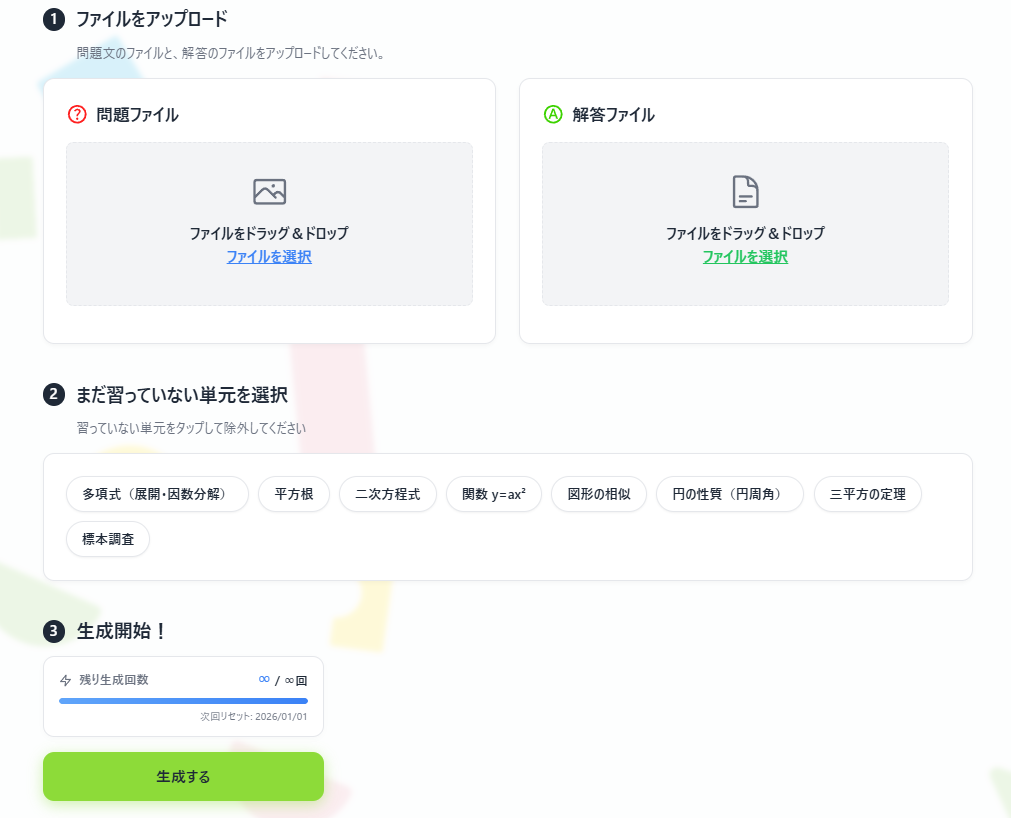
\includegraphics[width=\textwidth]{mongene-ui.png}
    \caption{モンジェネ\\問題生成画面}
    \label{fig:mongene_ui}
  \end{minipage}
\end{figure}

\noindent 図\ref{fig:grading_overview}--\ref{fig:grading_detail}に採点プロトタイプ「ScoGene」の画面を示す。問題文と答案のみを入力し（模範解答は渡していない状態でも）、LLMが自力で正答を計算し、手書き答案を正確に読み取る。正誤判定、途中式評価、部分点の理由、改善アドバイスを構造化して出力する。図\ref{fig:mongene_ui}はモンジェネの問題生成画面である。

% ============================================================
\section{提案者の腕前を証明できるもの}

本チームは、ドメイン知識（塾講師5年）、フルスタック開発力、デザイン力、AI/MLエンジニアリングの4つの専門性がバランスよく揃った構成である。全員が経産省AKATSUKI事業 ETSUZANの採択者であり、開発・発表の実績を持つ。

\begin{graybox}
\small\sffamily
\textbf{ETSUZAN Makers：}\url{https://meikan.etsuzan.org/}\\
\textbf{ETSUZAN最終報告会：}モンジェネ \url{https://youtu.be/PCIbYSYGWrI}\\
\hspace{9.5em}SakeScope \url{https://youtu.be/noTHRUNfiwA}\\
\textbf{テレビ放映（舛田 独占取材）：}\url{https://youtu.be/LLsKAEKmDJ4}
\end{graybox}

\begin{figure}[H]
  \centering
  \begin{minipage}[t]{0.42\textwidth}
    \centering
    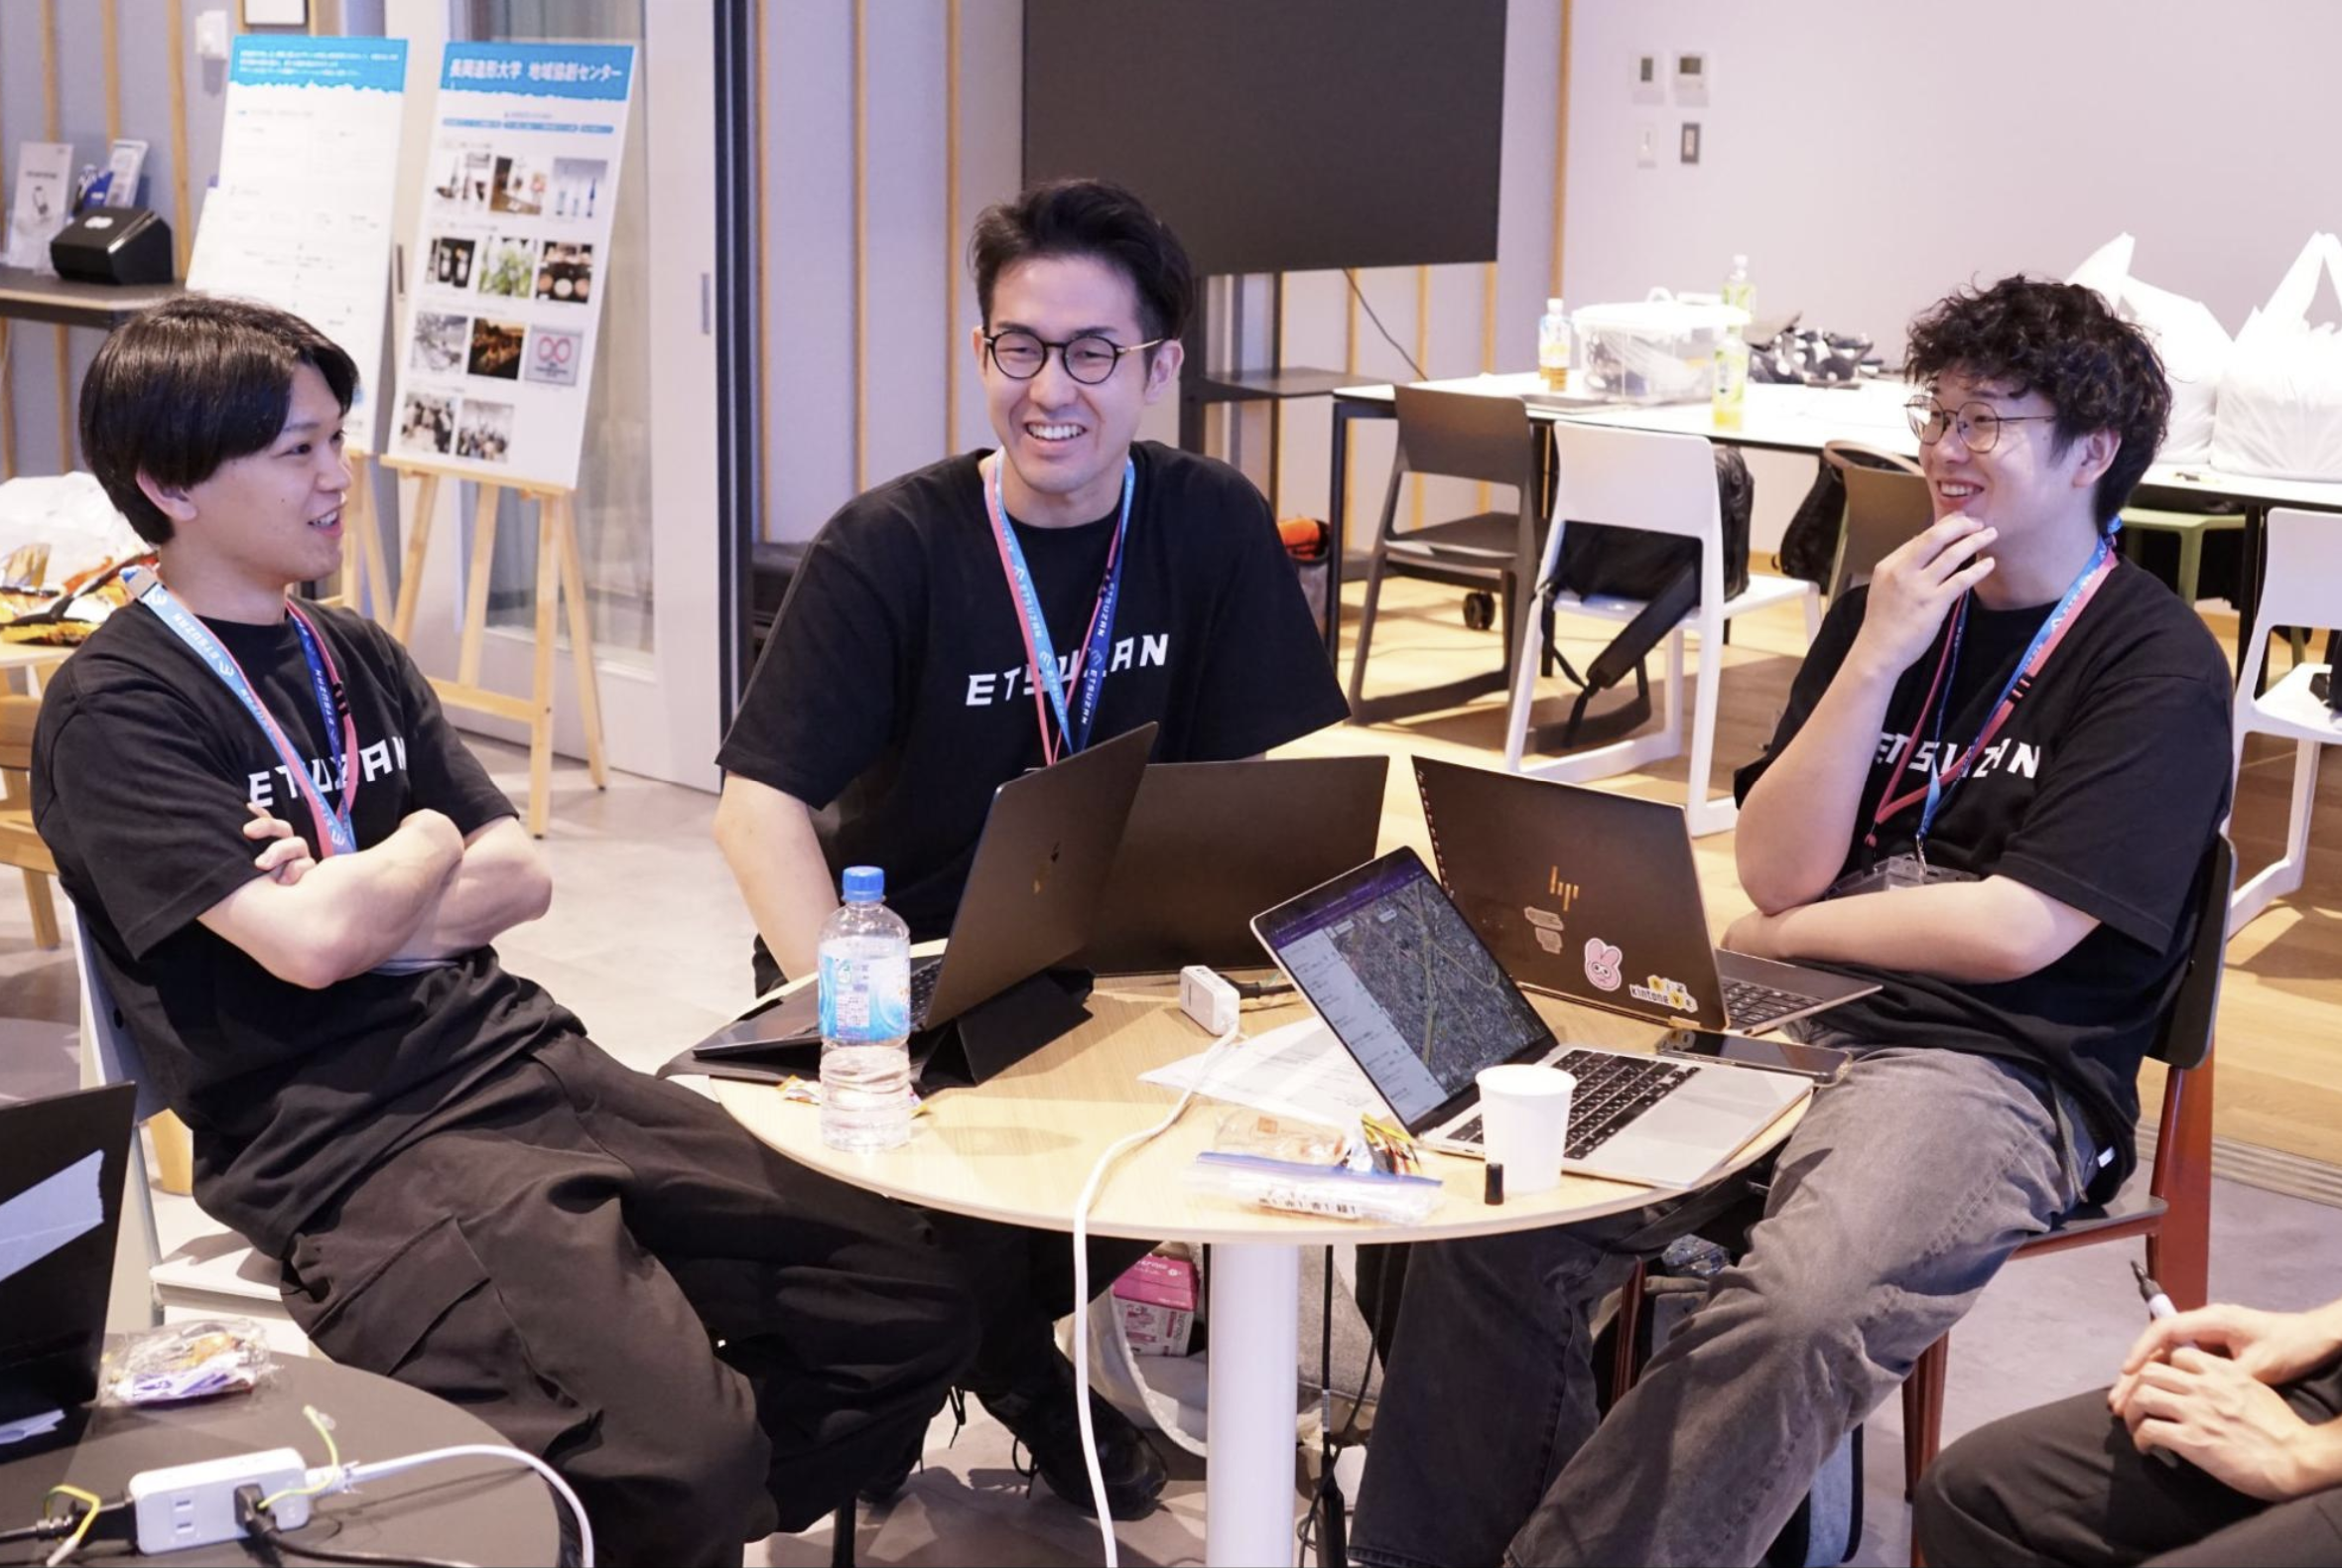
\includegraphics[width=\textwidth]{etsuzan-team.png}
    \caption{ETSUZANでの開発風景}
  \end{minipage}
  \hfill
  \begin{minipage}[t]{0.42\textwidth}
    \centering
    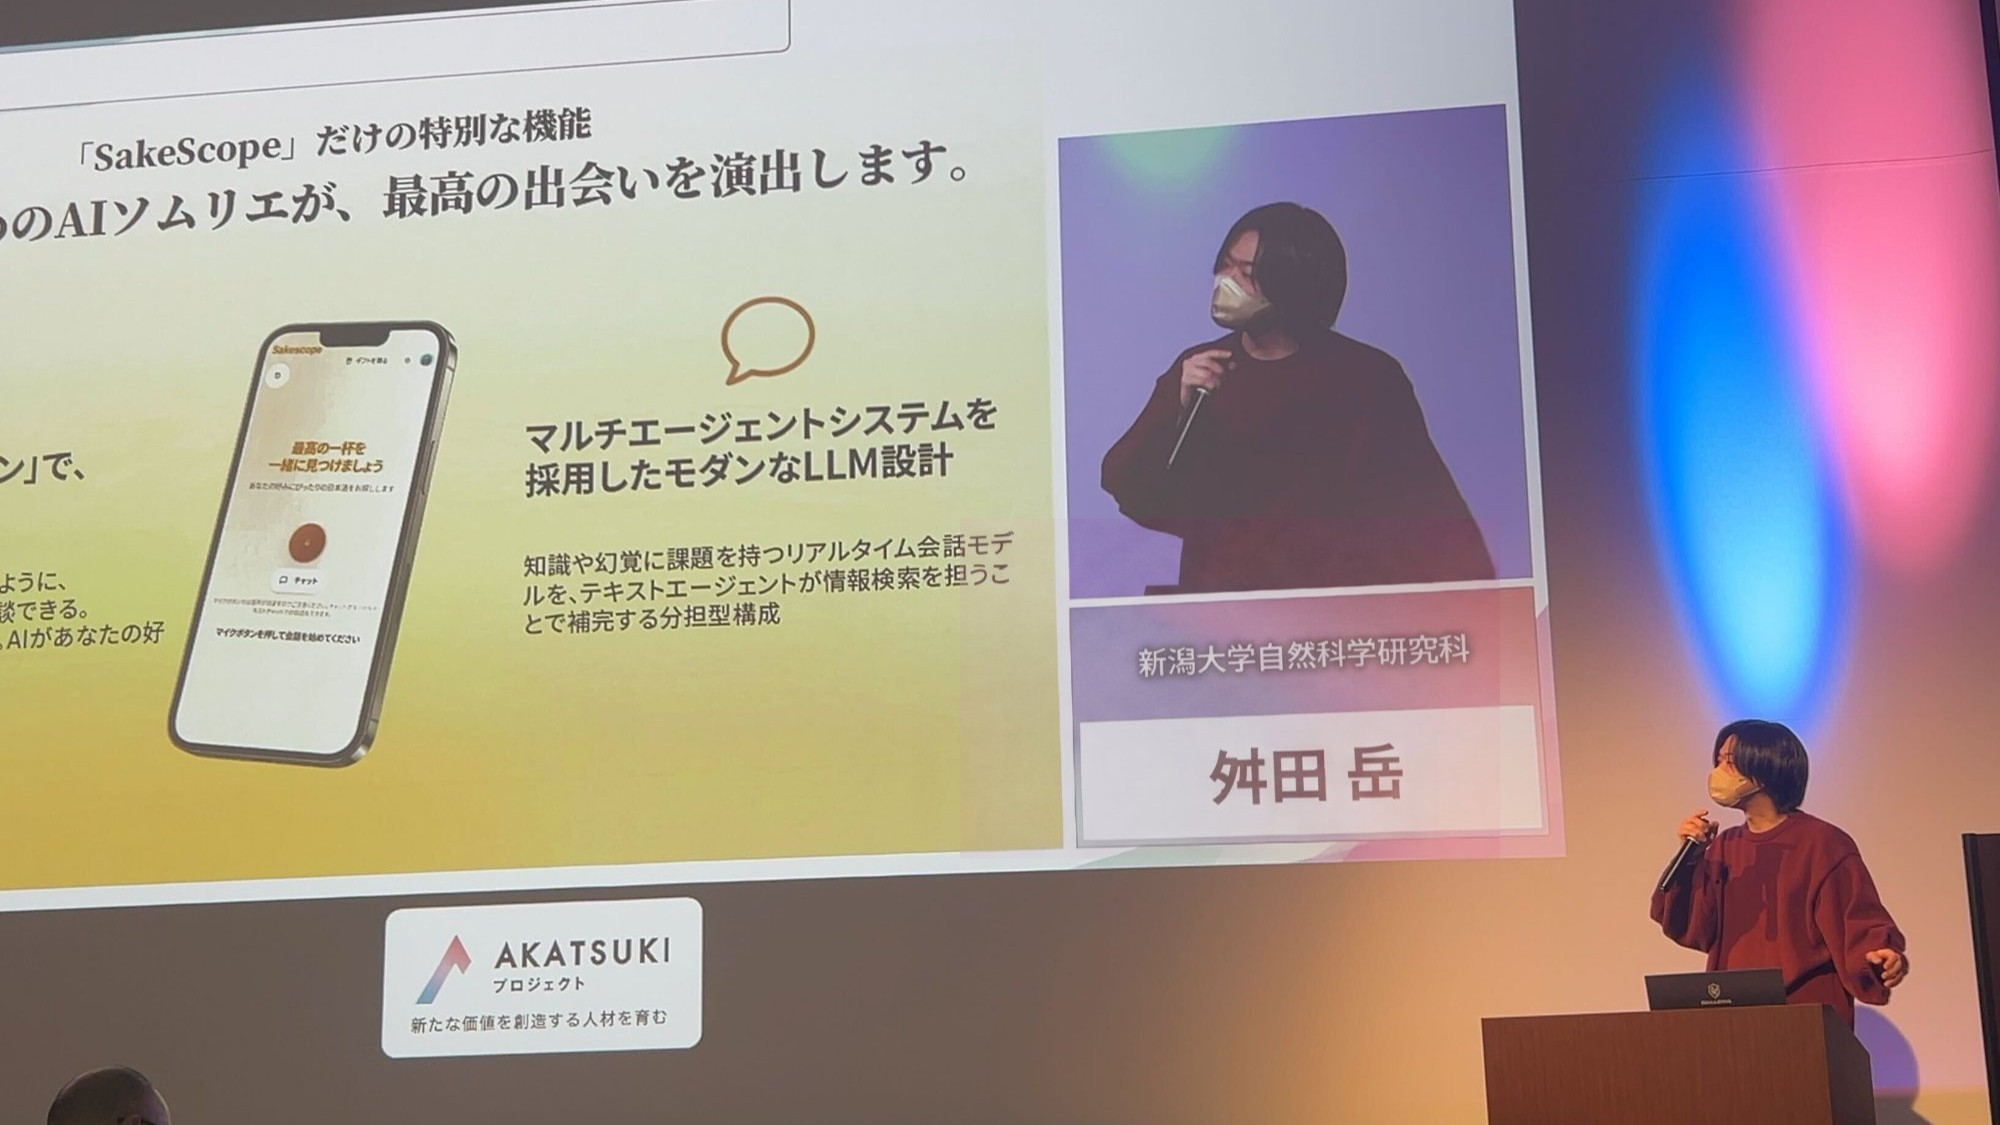
\includegraphics[width=\textwidth]{akatsuki-masuda.jpg}
    \caption{AKATSUKIカンファレンスで\\舛田が代表登壇}
  \end{minipage}
\end{figure}

\subsection*{高橋 創真（チーム代表）}

\begin{itemize}
  \item \textbf{塾講師5年目}：新潟県長岡市の個別指導塾で小学生から高校3年生まで理系科目を指導。現在は\textbf{講師80名を統括するリーダー}として塾の運営に携わる。本プロジェクトの課題は自身の現場経験から生まれた。
  \item \textbf{モンジェネ企画・開発}（ETSUZAN）：塾講師としての課題意識から無限問題生成AI「モンジェネ」を企画し、チームを率いて開発。
  \item \textbf{学園祭実行委員長}：長岡技術科学大学「技大祭」第43回実行委員長。約200名の組織を統率し、過去最大規模の成功に導いた。
  \item \textbf{NHK高専ロボコン}：4年間出場。チームリーダー兼部長として本田技研工業特別賞を受賞。
\end{itemize}

\subsection*{若月 耕紀（フルスタックエンジニア）}

\begin{itemize}
  \item \textbf{モンジェネ開発}（ETSUZAN）：LLMで数学問題を無限生成するWebアプリの設計・実装を主担当。
  \item \textbf{長岡インターンシップサイト}（業務委託）：要件定義からデプロイまでを1.5ヶ月で完遂。
  \item \textbf{NUTMEG}：学園祭を支えるアプリ群（Next.js, Rails）の開発団体代表。
  \item \textbf{修士研究}：「GraphVAEを用いたSlackチャットログに基づく組織構造再構成」（機械学習理論研究室）
\end{itemize}

\subsection*{小武 壮太（デザイナー）}

\begin{itemize}
  \item \textbf{モンジェネのUI設計}（ETSUZAN）：講師の認知負荷を下げるため、検索以外のフローをクリック操作のみで完結させるUI設計。生成AIでフロントエンドコードを出力・検証し、エンジニアとのイメージ共有を円滑化。
  \item \textbf{NUTMEG}：学内団体管理システム「GM2」のフロントエンド実装（Vue.js, TypeScript）。
\end{itemize}

\subsection*{舛田 岳（AI/MLエンジニア）}

\begin{itemize}
  \item \textbf{マーケティングAIエージェント}（株式会社b\&q）：100以上のツールを統合するMulti-Agent Architecture設計・実装。
  \item \textbf{SEO記事生成SaaS}（株式会社新大陸）：テックリードとしてLLM活用の記事自動生成システムを開発。月間数千記事の生成実績。
  \item \textbf{SakeScope}（ETSUZAN）：マルチモーダルLLMによるAI日本酒ソムリエ。テレビで独占取材・放映。
  \item \textbf{修士研究}：「進化的群知能に基づくLLMエージェント集団の協調最適化」（計算知能研究室）
\end{itemize}

% ============================================================
\section{プロジェクト遂行にあたっての特記事項}

高橋・若月・小武は長岡技術科学大学大学院 情報・経営システム工学分野 修士1年、舛田は新潟大学大学院 自然科学研究科 修士1年に所属し、来年度修士2年に進級予定である。全員が授業単位を取得済みであり、修士研究を抱えるのみである。研究室の指導教員との関係も良好で、未踏への応募についても容認されている。

開発場所は長岡技術科学大学工学研究科 機械学習理論研究室居室、および新潟大学自然科学研究科 計算知能研究室を使用する。高橋は塾に週複数日出勤しており、開発と実証実験のサイクルを高速に回すことが可能である。プロジェクト遂行に支障をきたす可能性は極めて低い。

\noindent\textbf{チームの経緯：}高橋・若月・小武は長岡技術科学大学の同期であり、学園祭実行委員会（NUTMEG）での開発活動を通じて技術的な信頼関係を構築した。舛田は新潟大学の大学院生で、経産省AKATSUKI事業 ETSUZANにて新潟県の同期採択者として出会い、互いのプロジェクト（モンジェネ・SakeScope）を通じて協力関係を深めた。全員がETSUZAN修了生であり、開発・発表を共にした仲間である。

% ============================================================
\section{IT以外の勉強、特技、生活、趣味}

\noindent\textbf{高橋 創真}：野球。小学3年から現在まで軟式野球部に所属し、地域ナイター杯で準優勝（5番レフト）。厳しい練習で培った粘り強さがプロジェクト推進の原動力。
\textbf{若月 耕紀}：動物鑑賞。実家が動物病院で犬9匹・猫6匹に囲まれて育った。言葉の通じない相手の裏側を想像する力がマネジメントスキルの基盤。
\textbf{小武 壮太}：デザイン制作。技大祭の広報としてInstagram運用を担当。「相手の想いを翻訳する力」がUI/UX設計を支える。
\textbf{舛田 岳}：バレーボール（JOC秋田県選抜）と映像制作。「何を、どう見せれば伝わるか」を考える力を培った。

% ============================================================
\section{将来のITについて思うこと・期すること}

AIの発展により様々な業務が効率化され、省人化・無人化された領域も多い。教育においてもAIの活用は急速に進んでいるが、教育と人は切り離すことができないと私たちは考える。

しかし、生徒の\textbf{モチベーション管理}はAIが踏み込めない領域だと考える。感情、人間関係、そして\textbf{憧れや夢を抱かせること}は機械にはできない。

\textbf{「憧れや夢は、人と人との関わりのなかで創発する。」}---だからこそ教育ITは、\textbf{Human-in-the-Loop}のシステムでなくてはならない。モンジェネは、AIが講師を\textbf{置き換える}のではなく、講師が生徒と向き合う時間を\textbf{最大化する}ためのツールである。採点や問題探しをAIに任せ、解説・動機づけ・進路相談といった「人にしかできない教育」に講師が集中できる世界を実現したい。

% ============================================================
\begin{small}
\noindent\textbf{参考文献}
\begin{enumerate}[leftmargin=2em,label={[\arabic*]}]
  \item Bloom, B.\,S. (1984). The 2 Sigma Problem. \textit{Educational Researcher}, 13(6), 4--16.
  \item Raman, S.\,K. (2025). Generative AI as a Solution to the 2-Sigma Problem and Equity in Higher Education. \textit{ResearchGate}.
  \item Corbett, A.\,T. \& Anderson, J.\,R. (1994). Knowledge Tracing. \textit{User Modeling and User-Adapted Interaction}, 4, 253--278.
  \item Cho, Y.\,et~al. (2024). A Systematic Review of Knowledge Tracing and Large Language Models in Education. \textit{arXiv:2412.09248}.
  \item Newman, M.\,A. (1977). An Analysis of Sixth-Grade Pupils' Errors on Written Mathematical Tasks.
  \item Wang, S.\,et~al. (2024). Large Language Models for Education: A Survey and Outlook. \textit{arXiv:2403.18105}.
  \item L\'{e}tourneau, A.\,et~al. (2025). A Systematic Review of AI-Driven ITS in K-12 Education. \textit{npj Science of Learning}, 10, 29.
  \item Otieno, H.\,et~al. (2025). Leveraging LLMs to Identify and Classify Student Errors Using the STACK Dataset. \textit{ResearchGate}.
\end{enumerate}
\end{small}

\end{document}
